\documentclass{article}

\usepackage[utf8]{inputenc}
\usepackage{graphicx}		% Graphics.
\usepackage{color}
\usepackage[english]{babel}
\usepackage{float}
\usepackage{subcaption}
\usepackage{xfrac}
\usepackage{matlab-prettifier}
\usepackage{amsmath}    
\usepackage{amssymb}
\usepackage{siunitx}
\usepackage{pdfpages}
\usepackage{longtable}

% Create a separate table for the appendix.
\usepackage[toc,page]{appendix}

% Table of Content has fast links to sections.
\usepackage{hyperref}

% Remove dots in table of contents.
\usepackage[titles]{tocloft}
\renewcommand{\cftdot}{}

% Page style.
\usepackage[top=2cm, bottom=2cm, left = 2cm, right = 2cm]{geometry}
\setlength{\parindent}{0pt}	% Disable indents.

\begin{document}

%----------------------------------------------------------------------------------------
%	Title page.
%----------------------------------------------------------------------------------------
%----------------------------------------------------------------------------------------
%	TITLE PAGE.
%----------------------------------------------------------------------------------------

\begin{titlepage} % Suppresses displaying the page number on the title page and the subsequent page counts as page 1.
	\center % Centre everything on the page.
	\newcommand{\HRule}{\rule{\linewidth}{0.5mm}} % Defines a new command for horizontal lines, change thickness here.
	
	
	%------------------------------------------------
	%	Logo.
	%------------------------------------------------
	
\includegraphics[width=0.4\textwidth, trim=0 0 0 -2cm]{figures/LTU_logo.jpg}\\[1cm]
		
	
	%------------------------------------------------
	%	Headings.
	%------------------------------------------------
	\textsc{\Huge Lule\aa \ University of Technology}\\[1.5cm]
	
	\textsc{\LARGE Atmospheric Physics}\\[0.3cm]
	
	\textsc{\large F7004R}\\[0.5cm]
	
	
	%------------------------------------------------
	%	Title.
	%------------------------------------------------
	\HRule\\[0.4cm]
	
	{\Huge\bfseries Meteorological measurements radiosonde}\\[0.4cm]
	
	\HRule\\[1.5cm]
	
	
	%------------------------------------------------
	%	Author & supervisor.
	%------------------------------------------------
	\begin{minipage}{0.4\textwidth}
		\begin{flushleft}
			\large
			\textit{Authors}\\
			E.F.M. Weterings
			D. Talavera
		\end{flushleft}
	\end{minipage}
	~
	\begin{minipage}{0.4\textwidth}
		\begin{flushright}
			\large
			\textit{Supervisors}\\
			V. Barabash\\
			M. Milz
		\end{flushright}
	\end{minipage}
	
	
	%------------------------------------------------
	%	Date.
	%------------------------------------------------
	\vfill\vfill\vfill % Position the date 3/4 down the remaining page.
	
	{\large\today} % Date, change the \today to a set date if you want to be precise.
	
	
\end{titlepage}


%----------------------------------------------------------------------------------------
%	TABLE OF CONTENT.
%----------------------------------------------------------------------------------------
\newpage				% Start at new page.
\pagenumbering{arabic}	% Page numbering reset & style.
\renewcommand{\contentsname}{Table of Contents}
\tableofcontents		% Add table of content.


%----------------------------------------------------------------------------------------
%	QUESTION 1.
%----------------------------------------------------------------------------------------
\newpage
\section{Find Station No. 03808. Which location is this station attributed to? Where is it situated?}
As can be seen from figure \ref{fig:1}, the grounstation 03808 is located in south west part of England, more specifically in Camborne. 

\begin{figure}[H]
	\centering
 	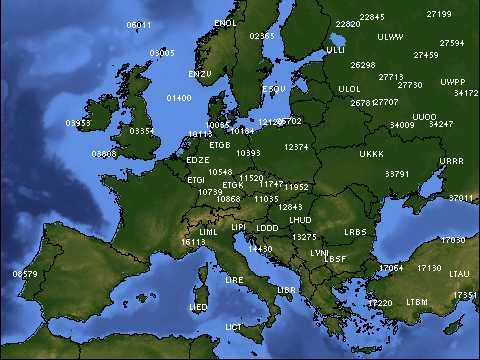
\includegraphics[width=1\textwidth]{figures/europe.jpg}
 	\caption{Europa weather stations.}
 	\label{fig:1}
\end{figure}


%----------------------------------------------------------------------------------------
%	QUESTION 2.
%----------------------------------------------------------------------------------------
\section{Extract the radiosonde profile data for 2007-07-05 0:00 UTC, 12:00 UTC and 2007-07-06 0:00 UTC}
% http://weather.uwyo.edu/cgi-bin/sounding?region=europe&TYPE=TEXT%3ALIST&YEAR=2007&MONTH=07&FROM=0500&TO=0600&STNM=03808
The information can be found online by clicking on the following URL:\\
http://weather.uwyo.edu/cgi-bin/sounding?region=europe\&TYPE=TEXT\%3ALIST\&YEAR=2007\&MONTH=07\\
\&FROM=0500\&TO=0600\&STNM=03808\\

The information can also be found on the next page.
% Table generated by Excel2LaTeX from sheet 'Sheet1'
% Table generated by Excel2LaTeX from sheet 'Sheet1'
% Table generated by Excel2LaTeX from sheet 'Sheet1'
% Table generated by Excel2LaTeX from sheet 'Sheet1'
\small{\begin{longtable}[h!]{p{0.1\textwidth}|p{0.1\textwidth}|p{0.1\textwidth}|p{0.1\textwidth}|p{0.1\textwidth}|p{0.1\textwidth}|p{0.1\textwidth}|p{0.1\textwidth}|p{0.1\textwidth}|p{0.1\textwidth}}
    \multicolumn{1}{l}{HGHT [m]} & \multicolumn{1}{l}{TEMP [C]} & \multicolumn{1}{l}{DWPT [C] } & \multicolumn{1}{l}{RELH [\%]} & \multicolumn{1}{l}{MIXR [g/kg]} & \multicolumn{1}{l}{DRCT [deg]} & \multicolumn{1}{l}{SKNT [knot]} & \multicolumn{1}{l}{THAT [K]} & \multicolumn{1}{l}{ THTE [K]} & \multicolumn{1}{l}{THTV [K]} \\ \hline
      &   &   &   &   &   &   &   &   &  \\
    88 & 13.6 & 11.1 & 85 & 8.3 & 290 & 15 & 286.2 & 309.5 & 287.6 \\
    104 & 13.6 & 11.2 & 85 & 8.37 & 290 & 17 & 286.3 & 309.8 & 287.8 \\
    143 & 13.4 & 11.1 & 86 & 8.36 & 290 & 20 & 286.6 & 310 & 288 \\
    194 & 12.9 & 10.8 & 87 & 8.25 & 290 & 25 & 286.6 & 309.8 & 288 \\
    270 & 12.2 & 10.4 & 89 & 8.1 & 290 & 26 & 286.6 & 309.4 & 288 \\
    520 & 9.9 & 9.2 & 96 & 7.72 & 290 & 31 & 286.7 & 308.4 & 288 \\
    572 & 9.4 & 9 & 97 & 7.64 & 290 & 31 & 286.7 & 308.3 & 288 \\
    686 & 8.4 & 8.4 & 100 & 7.43 & 290 & 32 & 286.8 & 307.8 & 288.1 \\
    793 & 7.8 & 7.8 & 100 & 7.22 & 290 & 32 & 287.3 & 307.7 & 288.5 \\
    1066 & 6.2 & 6.2 & 100 & 6.68 & 302 & 28 & 288.4 & 307.4 & 289.5 \\
    1130 & 6 & 6 & 100 & 6.66 & 305 & 27 & 288.8 & 307.9 & 290 \\
    1224 & 5.8 & 5.8 & 100 & 6.63 & 304 & 28 & 289.5 & 308.5 & 290.7 \\
    1461 & 4.4 & 4.4 & 100 & 6.18 & 300 & 29 & 290.4 & 308.3 & 291.5 \\
    1490 & 4.4 & 4.2 & 99 & 6.12 & 300 & 29 & 290.7 & 308.5 & 291.8 \\
    1519 & 4.2 & 3.6 & 96 & 5.88 & 300 & 29 & 290.8 & 307.9 & 291.9 \\
    1704 & 4.6 & -0.4 & 70 & 4.51 & 300 & 32 & 293.1 & 306.5 & 293.9 \\
    1733 & 4.6 & -0.6 & 69 & 4.46 & 300 & 32 & 293.4 & 306.7 & 294.2 \\
    1842 & 4.6 & -1.4 & 65 & 4.26 & 300 & 32 & 294.6 & 307.3 & 295.3 \\
    2127 & 2.6 & -1.7 & 73 & 4.32 & 300 & 34 & 295.4 & 308.4 & 296.2 \\
    2199 & 2.4 & -2.4 & 71 & 4.13 & 300 & 34 & 295.9 & 308.4 & 296.7 \\
    2272 & 3.2 & -4.8 & 56 & 3.48 & 300 & 34 & 297.6 & 308.2 & 298.2 \\
    2388 & 3 & -6.7 & 49 & 3.05 & 300 & 35 & 298.5 & 308 & 299.1 \\
    2549 & 2.6 & -9.4 & 41 & 2.53 & 299 & 35 & 299.8 & 307.8 & 300.3 \\
    3003 & -0.3 & -12.3 & 40 & 2.12 & 295 & 37 & 301.5 & 308.3 & 301.9 \\
    3060 & -0.7 & -12.7 & 40 & 2.07 & 295 & 37 & 301.7 & 308.3 & 302.1 \\
    3360 & -2.7 & -16.3 & 34 & 1.6 & 295 & 36 & 302.8 & 308 & 303.1 \\
    3611 & -4.3 & -19.3 & 30 & 1.28 & 295 & 38 & 303.7 & 307.9 & 303.9 \\
    3856 & -5.3 & -36.3 & 7 & 0.27 & 295 & 41 & 305.2 & 306.2 & 305.3 \\
    3880 & -5.5 & -36.5 & 7 & 0.27 & 295 & 41 & 305.3 & 306.3 & 305.4 \\
    4469 & -9.5 & -42.5 & 5 & 0.16 & 295 & 44 & 307.3 & 307.9 & 307.3 \\
    4589 & -10.4 & -43.5 & 5 & 0.14 & 295 & 45 & 307.6 & 308.1 & 307.6 \\
    4696 & -11.3 & -44.3 & 5 & 0.13 & 295 & 48 & 307.8 & 308.3 & 307.8 \\
    4915 & -11.6 & -41.4 & 6 & 0.18 & 295 & 53 & 309.9 & 310.6 & 310 \\
    5169 & -12 & -38 & 9 & 0.27 & 305 & 63 & 312.4 & 313.4 & 312.5 \\
    5241 & -12.1 & -37.1 & 11 & 0.3 & 303 & 66 & 313.1 & 314.3 & 313.2 \\
    5372 & -12.7 & -27.7 & 27 & 0.76 & 301 & 71 & 313.9 & 316.7 & 314.1 \\
    5401 & -12.9 & -27.1 & 29 & 0.8 & 300 & 72 & 314 & 316.9 & 314.2 \\
    5565 & -14.1 & -24.1 & 43 & 1.08 & 300 & 68 & 314.5 & 318.3 & 314.7 \\
    5670 & -14.7 & -25.7 & 39 & 0.95 & 300 & 66 & 315.1 & 318.4 & 315.2 \\
    5746 & -15.1 & -27.1 & 35 & 0.84 & 300 & 65 & 315.5 & 318.5 & 315.6 \\
    5776 & -15.4 & -26.7 & 38 & 0.88 & 300 & 64 & 315.5 & 318.6 & 315.6 \\
    6103 & -18.7 & -22 & 75 & 1.4 & 303 & 65 & 315.3 & 320.2 & 315.6 \\
    6327 & -20 & -24.1 & 70 & 1.19 & 305 & 65 & 316.4 & 320.6 & 316.6 \\
    6376 & -20.3 & -24.6 & 68 & 1.15 & 305 & 66 & 316.6 & 320.7 & 316.9 \\
    6657 & -21.9 & -39.9 & 18 & 0.27 & 305 & 73 & 318.1 & 319.1 & 318.1 \\
    7035 & -24.5 & -42.5 & 17 & 0.22 & 305 & 82 & 319.5 & 320.3 & 319.5 \\
    7158 & -24.8 & -49.1 & 9 & 0.11 & 305 & 85 & 320.7 & 321.1 & 320.7 \\
    7230 & -24.9 & -52.9 & 6 & 0.07 & 303 & 85 & 321.4 & 321.7 & 321.4 \\
    7320 & -25.3 & -58.3 & 3 & 0.04 & 300 & 85 & 322 & 322.2 & 322 \\
    7356 & -25.5 & -57 & 4 & 0.04 & 300 & 85 & 322.2 & 322.4 & 322.2 \\
    7393 & -25.7 & -55.7 & 4 & 0.05 & 301 & 85 & 322.4 & 322.6 & 322.4 \\
    7635 & -27.3 & -44.3 & 18 & 0.2 & 306 & 86 & 323.4 & 324.2 & 323.4 \\
    7824 & -28.7 & -43.4 & 23 & 0.22 & 310 & 86 & 324 & 324.9 & 324 \\
    8279 & -32.1 & -41.1 & 40 & 0.3 & 306 & 91 & 325.4 & 326.6 & 325.4 \\
    8380 & -33 & -40.9 & 45 & 0.31 & 305 & 92 & 325.5 & 326.8 & 325.6 \\
    8776 & -36.4 & -40 & 69 & 0.36 & 305 & 100 & 326.2 & 327.6 & 326.2 \\
    8863 & -37.1 & -39.8 & 76 & 0.37 & 306 & 101 & 326.3 & 327.8 & 326.4 \\
    8993 & -37.7 & -40.7 & 73 & 0.35 & 307 & 103 & 327.2 & 328.6 & 327.3 \\
    9305 & -40.1 & -47.1 & 47 & 0.18 & 310 & 107 & 328.1 & 328.9 & 328.1 \\
    9350 & -40.5 & -47.5 & 47 & 0.18 & 310 & 108 & 328.2 & 328.9 & 328.2 \\
    9395 & -40.8 & -47.3 & 49 & 0.18 & 310 & 108 & 328.4 & 329.1 & 328.4 \\
    9534 & -41.7 & -46.7 & 58 & 0.2 & 310 & 109 & 329 & 329.8 & 329.1 \\
    9769 & -42.9 & -50.9 & 41 & 0.13 & 310 & 110 & 330.6 & 331.1 & 330.6 \\
    10035 & -45.2 & -51.3 & 50 & 0.13 & 310 & 112 & 331 & 331.5 & 331 \\
    10185 & -46.5 & -51.5 & 57 & 0.13 & 313 & 119 & 331.2 & 331.8 & 331.3 \\
    10311 & -46.8 & -55.2 & 38 & 0.08 & 315 & 125 & 332.6 & 332.9 & 332.6 \\
    10337 & -46.9 & -55.9 & 35 & 0.08 & 315 & 125 & 332.8 & 333.1 & 332.8 \\
    10570 & -48.9 & -59.9 & 27 & 0.05 & 310 & 122 & 333.2 & 333.4 & 333.2 \\
    10623 & -49.1 & -59.1 & 30 & 0.05 & 310 & 122 & 333.7 & 333.9 & 333.7 \\
    10972 & -51.1 & -62.6 & 24 & 0.04 & 310 & 120 & 335.9 & 336.1 & 335.9 \\
    11084 & -51.7 & -63.7 & 22 & 0.03 & 310 & 118 & 336.6 & 336.7 & 336.6 \\
    11486 & -53.5 & -67.5 & 17 & 0.02 & 310 & 109 & 339.9 & 340 & 339.9 \\
    11820 & -52.9 & -70 & 11 & 0.01 & 310 & 103 & 346 & 346 & 346 \\
    11978 & -52.6 & -71.3 & 9 & 0.01 & 305 & 90 & 348.9 & 348.9 & 348.9 \\
    12010 & -52.5 & -71.5 & 8 & 0.01 & 305 & 89 & 349.5 & 349.5 & 349.5 \\
    12341 & -51.9 & -73.9 & 5 & 0.01 & 299 & 86 & 355.6 & 355.6 & 355.6 \\
    12584 & -51.3 & -77 & 3 & 0.01 & 295 & 83 & 360.4 & 360.5 & 360.4 \\

  \label{tab:addlabel}%
\end{longtable}}%




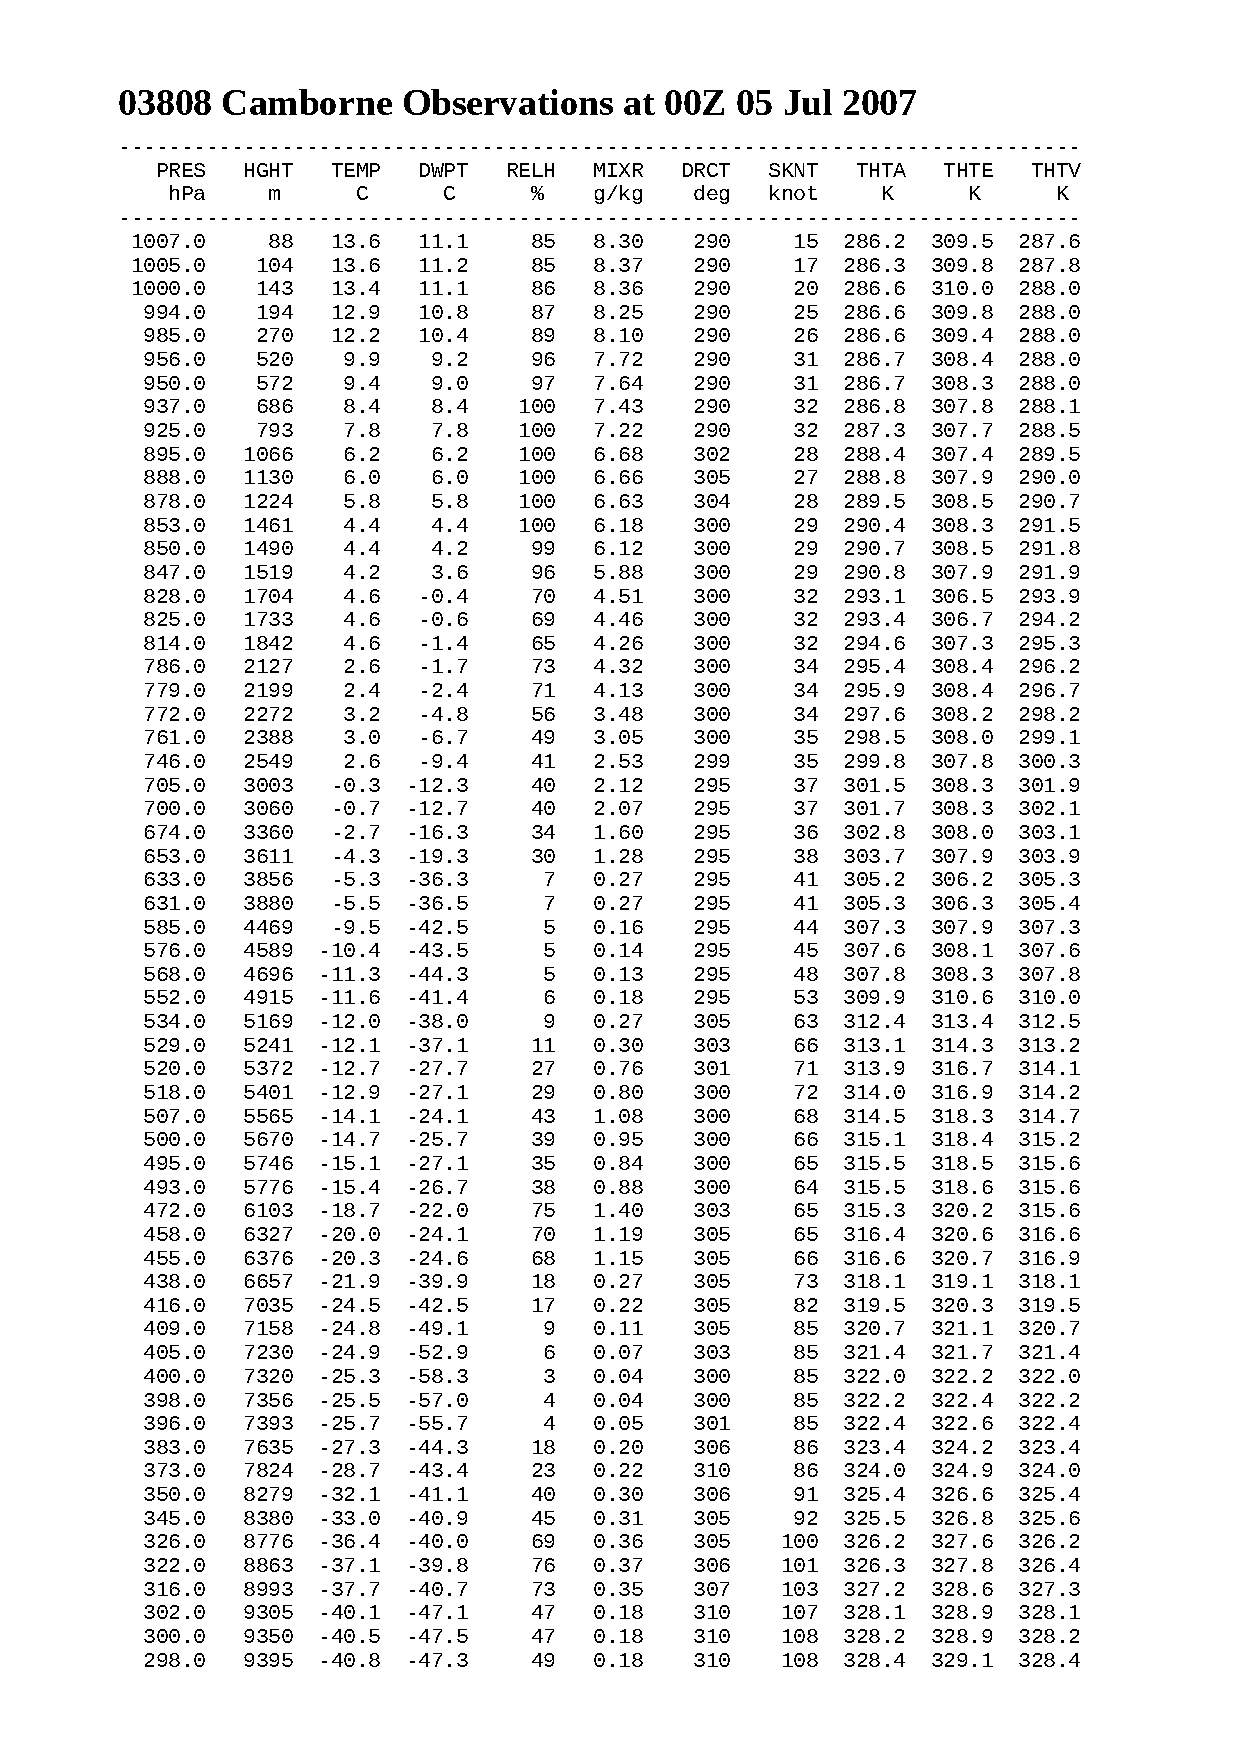
\includepdf[pages=-]{figures/Radiosonde-Data.pdf}


%----------------------------------------------------------------------------------------
%	QUESTION 3.
%----------------------------------------------------------------------------------------
\newpage
\section{Plot the profiles of temperature T, dewpoint temperature $T_D$ and relative humidity RH for each of theses dates. (T and $T_D$ in one plot, RH in a separate one) Use a suitable altitude coordinate!}



%----------------------------------------------------------------------------------------
%	QUESTION 4.
%----------------------------------------------------------------------------------------
\newpage
\section{How are T and $T_D$ related to each other? Consider RH for your argumentation}



%----------------------------------------------------------------------------------------
%	QUESTION 5.
%----------------------------------------------------------------------------------------
\newpage
\section{At which altitude for these data is the tropopause height located?What method do you use to determine the tropopause?}


%----------------------------------------------------------------------------------------
%	QUESTION 6.
%----------------------------------------------------------------------------------------
\newpage
\section{Describe the some crucial differences between the tropospheric parts of the above plotted profiles. What did probably happen during that date?}



%----------------------------------------------------------------------------------------
%	QUESTION 7.
%----------------------------------------------------------------------------------------
\newpage
\section{Plot the data for 2007-07-05, 12:00 UTC as Stuve diagram. What does the Stuve diagram show? What do the different “help lines” mean. What is this type of diagram used for? Use internet resources to find out}


\end{document}
